\documentclass[12pt]{article}
\usepackage[margin=1in, a4paper]{geometry}

\title{Document Template in Latex}
\author{Firuza Aibara}

 \ifx\pdftexversion\undefined
 \usepackage[dvips]{graphicx}
 \else
 
 \usepackage[pdftex]{graphicx}
 \DeclareGraphicsRule{*}{mps}{*}{}
 \fi
\usepackage{url}
\usepackage{chapterbib}
\usepackage{hyperref}
\usepackage{lscape}
\usepackage{longtable}
\usepackage{float}
\usepackage{url}
\usepackage{multicol}
\usepackage{color}

\usepackage{fancyhdr}
\pagestyle{fancy}
\lhead{\leftmark}
\rhead{}
\lfoot{Amit, Harshit, Mridul, Ritik,\\ Soumyakant}
\cfoot{\today}
\rfoot{\thepage}

\renewcommand{\bibname}{References}

\setcounter{secnumdepth}{4}
\setcounter{tocdepth}{4}

\begin{document}

\begin{titlepage}
 \begin{center}
\Huge
\textbf{Configurable and Scalable IITBombayX MOOC platform on commodity servers} \\
\vfill
\LARGE
\textbf{Amit Kumar Tiwari, Harshit Mogalapalli, Mridul Mahajan, Ritik Kumar,\\ Soumyakant Mohakul}\\
\vfill
\Large
Last Updated: \today
\end{center}
\end{titlepage}

 \pagebreak \textcolor{white}{text} \pagebreak
\thispagestyle{empty}

\pagebreak
\setcounter{page}{1}
\pagenumbering{roman}

\listoffigures

\pagebreak

\listoftables

\pagebreak

\tableofcontents

\pagebreak

\setcounter{page}{1}
\pagenumbering{arabic}


\section{Introduction}

The aim of this project is to deploy an instance of Open edX MOOC platform on a multi-node cluster using Kubernetes as a container orchestrator. \\

\textbf{Technologies used:}
\begin{itemize}
	\item Docker
	\item Kubernetes
	\item Ansible
	\item Shell scripting
	\item Git
	\item Cluster management and configuration
\end{itemize}
%Paste appropriate content from here. 

%The following is an example of inserting an image which is shown in Figure ~\ref{fig:Image1} 

%\begin{figure}[hb]
 %\centering
 %
\includegraphics[width=12cm]{./Image1.jpg}
 %\caption{Name of the Figure\label{fig:Image1}}
%\end{figure}

\section{Open edX}
Open edX is an open source online MOOC provider. It provides both web and mobile platforms to clone the basic template of e-learning platform. In this project, we are working on the web platform.

\subsection{Releases}
Open edX has multiple releases. Some of the prominent ones are:
\begin{itemize}
	\item Ironwood
	\item Hawthorn
	\item Ginkgo
\end{itemize}
We are using the Ironwood.1 release in this project.

\subsection{Installation}
There are two ways to install Open edX:
\begin{itemize}
	\item Native installation
	\item Docker-based installation
\end{itemize}
\subsubsection{Native installation}
Write text here.  
\subsubsection{Docker-based installation}
	\label{sec:dockerinstall}
	\textbf{i) Installing docker engine, docker machine and docker compose:}
	\\ \\
	The docker based installing allows the resources of your system to be utilized in an optimal way. Docker is based on the principle of containerization. For proper working of the devstack we need the Docker engine, docker machine and docker compose. We shall install each of them one after another.\\ \\
	For installing the docker engine the following commands need to be run:
	\begin{enumerate}
		\item sudo apt-get update
		\item sudo apt-get install \ \\
		apt-transport-https \
		ca-certificates \
		curl \
		gnupg-agent \
		software-properties-common
		\item curl -fsSL https://download.docker.com/linux/ubuntu/gpg | sudo apt-key add -
		\item sudo apt-key fingerprint 0EBFCD88
		\item sudo add-apt-repository \ \\
		"deb [arch=amd64] https://download.docker.com/linux/ubuntu \ \\
		\$(lsb\_release -cs) \ \\
		stable"
		\item sudo apt-get update
		\item sudo apt-get install docker-ce docker-ce-cli containerd.io
		\item apt-cache madison docker-ce
		\item sudo apt-get install docker-ce=$<VERSION\_STRING>$\\docker-ce-cli=$<VERSION\_STRING>$ containerd.io
	\end{enumerate}
	\textbf{In order to test the successfull installation of Docker, run the following \\command:\\}
	sudo docker run hello-world\\\\
	For installing the docker machine the following command needs to be run:\\ \\
	base=https://github.com/docker/machine/releases/download/v0.16.0 \ \&\& \\
	curl -L \$base/docker-machine-\$(uname -s)-\$(uname -m)$>$/tmp/docker-machine \ \&\& \\
	sudo install /tmp/docker-machine /usr/local/bin/docker-machine\\ \\
	For installing docker compose the following commands need to be followed:
	\begin{enumerate}
		\item sudo curl -L "https://github.com/docker/compose/releases/download/1.24.0/docker-compose-\$(uname -s)-\$(uname -m)" -o /usr/local/bin/docker-compose
		\item sudo chmod +x /usr/local/bin/docker-compose
	\end{enumerate}
	For checking the successful installation of all the above you can use the \ -\ -version flag with the corresponding command to check the installed version.\\\\\\\\\\\\
	\textbf{ii) Installing Ironwood Devstack:} \\ \\
	Devstack comes with different variations as per the different versions. The three popular versions of the devstack are Ginkgo, Hawthron and Ironwood. \\\\
	The following commands perform the Ironwood-release installation of the devstack:
	\begin{enumerate}
		\item git clone https://github.com/edx/devstack
		\item cd devstack
		\item git checkout open-release/ironwood.master
		\item export OPENEDX\_RELEASE=ironwood.master
		\item make dev.checkout
		\item make dev.clone
		\item make dev.provision
	\end{enumerate}
	On successfully running dev.provision you will have 15 docker-containers running. The list of them can be obtained using command:  docker ps
	\\\\
	The list of docker-containers are: \href{https://drive.google.com/open?id=0B168SrnPp4BpZ1RCQ1VncU81VEZYanl2SUNWN2dtRUg1bGRv}{Docker-containers List}
	\\\\
	The Provision Log for the tasks executed are: \href{https://drive.google.com/open?id=0B168SrnPp4BpclQ3d3gwbDNWLWtrUzduYUt6Vko4S2h6bzBz}{provision.log}
	
	
\section{Docker}
\subsection{About Docker}
Docker is an open-source software tool designed to automate and ease the process of creating, packaging, and deploying applications using an environment called a container. The use of Linux containers to deploy applications is called containerization. A Container allows us to package an application with all of the parts needed to run an application (code, system tools, logs, libraries, configuration settings and other dependencies) and sends it out as a single standalone package deployable via \href{https://goo.gl/f77a2v}{Ubuntu} (in this case 16.04 LTS). Docker can be installed on \href{https://goo.gl/iTES81}{other platforms} as well. Currently, the Docker software is maintained by the Docker community and Docker Inc. Check out the \href{https://docs.docker.com/}{official documentation} to find more specifics on Docker. Docker Terms and Concepts. 
\subsection{Terms related to Docker}
\subsubsection{Containerization}
Containerization is a lightweight alternative to full machine virtualization (like VMWare) that involves encapsulating an application within a container with its own operating environment.
\subsubsection{Docker Image}
A \textit{Docker Image} is the basic unit for deploying a Docker container. A Docker image is essentially a static snapshot of a container, incorporating all of the objects needed to run a container.
\subsubsection{Docker Container}
A \textit{Docker Container} encapsulates a Docker image and when live and running, is considered a container. Each container runs isolated in the host machine.
\subsubsection{Docker Registry}
The \textit{Docker Registry} is a stateless, highly scalable server-side application that stores and distributes Docker images. This registry holds Docker images, along with their versions and, it can provide both public and private storage location. There is a public Docker registry called \href{https://hub.docker.com/}{Docker Hub} which provides a free-to-use, hosted Registry, plus additional features like organization accounts, automated builds, and more. Users interact with a registry by using Docker push or pull commands.
\subsubsection{Docker Engine}
The \textit{Docker Engine} is a layer which exists between containers and the Linux kernel and runs the containers. It is also known as the Docker daemon. Any Docker container can run on any server that has the Docker-daemon enabled, regardless of the underlying operating system.
\subsubsection{Docker Compose}
\textit{Docker Compose} is a tool that defines, manages and controls multi-container Docker applications. With Compose, a single configuration file is used to set up all of your application’s services. Then, using a single command, you can create and start all the services from that file
\subsubsection{Dockerfiles}
Dockerfiles are merely text documents (.yaml files) that contains all of the configuration information and commands needed to assemble a container image. With a Dockerfile, the Docker daemon can automatically build the container image.
\subsection{Docker-Machine}
Write text here
\subsection{Docker-Compose}
Docker compose is a tool to define and run docker applications using multiple containers. The services of the applications can be configured using a YAML file which is by default named as docker-compose.yml. Docker compose enables the users to create and start all the services from the configuration file with a single command.
\subsection{Docker Swarm}
Write text here
\section{Ansible}
\subsection{Installing openssh}
\$ sudo apt-get install openssh-server\\
\$ sudo apt-get install openssh-client
\subsection{Generating key at server and copying in client}
\$ ssh-keygen (generate ssh-key)\\
Copy this key to all nodes so that you don’t have to enter a password each time while connecting to the node.\\
To copy ssh-key type command:\\
\$ ssh-copy-id $username@IP\_address$
\subsection{Ansible setup}
\subsubsection{Adding repository}
\$ sudo apt-add-repository ppa:ansible/ansible\\
\$ sudo apt-get update
\subsubsection{Installing ansible}
\$ sudo apt-get install ansible
\subsubsection{Checking version}
\$ ansible  --version
\subsubsection{Ansible directories}
\$ ls -lha /etc/ansible/
\subsubsection{Making a copy a directory for our use}
\$ cp -R /etc/ansible/ myplatform\\
vi ansible.cfg (uncomment the inventory =  hosts)\\
vi hosts (remove all and write all nodes in new line)\\\\
\textbf{You can check if all the nodes working by running:}\\
\$ ansible -m ping all
\subsection{Some useful commands for ansible}
\subsubsection{To see the hostnames of all nodes}
\$ ansible -m shell -a 'hostname' all
\subsubsection{To see the volumes used by all nodes}
\$ ansible -m shell -a 'df -h' all
\subsubsection{To run an ansible-playbook}
\$ ansible-playbook  -K playbook-docker.yml
\section{Kubernetes}
\subsection{What is Kubernetes}
Kubernetes is a container-orchestration tool developed by Google in 2015 and later donated to CNCF (Cloud Native Computing Foundation). Kubernetes provides a smart way for orchestration in setting a multi-node cluster. Kubernetes comes with a lot of functionalities such as load balancing, pod scaling, process scheduling and process management.
\subsection{Main Features Of Kubernetes}
\begin{itemize}
	\item \href{https://kubernetes.io/docs/concepts/services-networking/service/}{Service discovery and load balancing}
	\item \href{https://kubernetes.io/docs/concepts/storage/persistent-volumes/}{Storage orchestration}
	\item \href{https://kubernetes.io/docs/concepts/configuration/manage-compute-resources-container/}{Automatic bin packing}
	\item \href{https://kubernetes.io/docs/concepts/workloads/controllers/replicationcontroller/#how-a-replicationcontroller-works}{Self-healing}
	\item \href{https://kubernetes.io/docs/concepts/workloads/controllers/deployment/}{Automated rollouts and rollbacks}
	\item \href{https://kubernetes.io/docs/concepts/configuration/secret/}{Secret and configuration management}
	\item \href{https://kubernetes.io/docs/concepts/workloads/controllers/jobs-run-to-completion/}{Batch execution}
	\item \href{https://kubernetes.io/docs/tasks/run-application/horizontal-pod-autoscale/}{Horizontal scaling}
\end{itemize}
\subsection{Terminologies in Kubernetes}
\subsubsection{Pod}
The most fundamental unit in a kubernetes cluster is a pod. A pod is a collection of container and volumes. Each pod has an IP address.\\
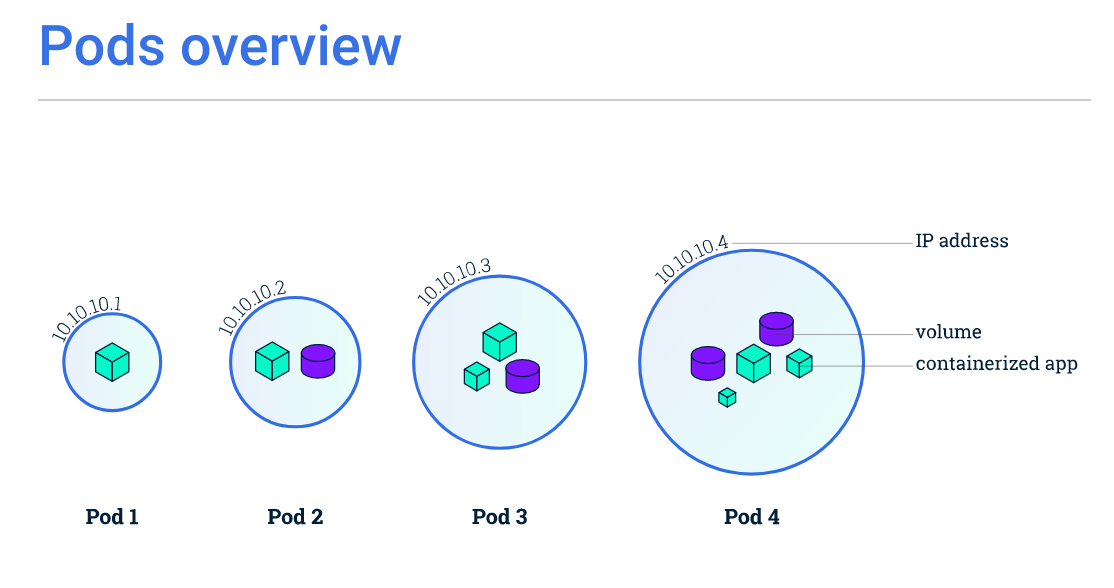
\includegraphics[width=\textwidth, trim= 0 0 0 5cm, clip=true]{pods}
\subsubsection{Deployment}
A deployment can be seen as a stateless state of the pod. A deployment is used to provide pod definition and rolling updates to the pod. A deployment contains information such as number of replicas, image, volume mount, hostname and restart policy.\\
\begin{center}
	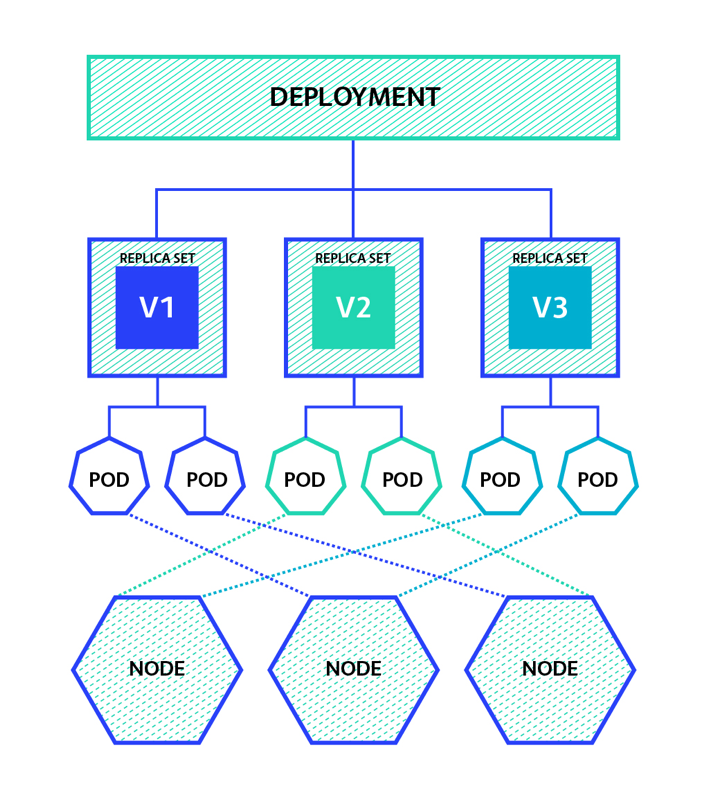
\includegraphics[totalheight=0.45\textheight]{deploy}
\end{center}
\subsubsection{Service}
A service exposes a deployment as a network service. A deployment is stateless whereas a service can be considered as a stateful definition. The three types of services in kubernetes are: ClusterIP, NodePort and LoadBalancer.\\
\begin{center}
	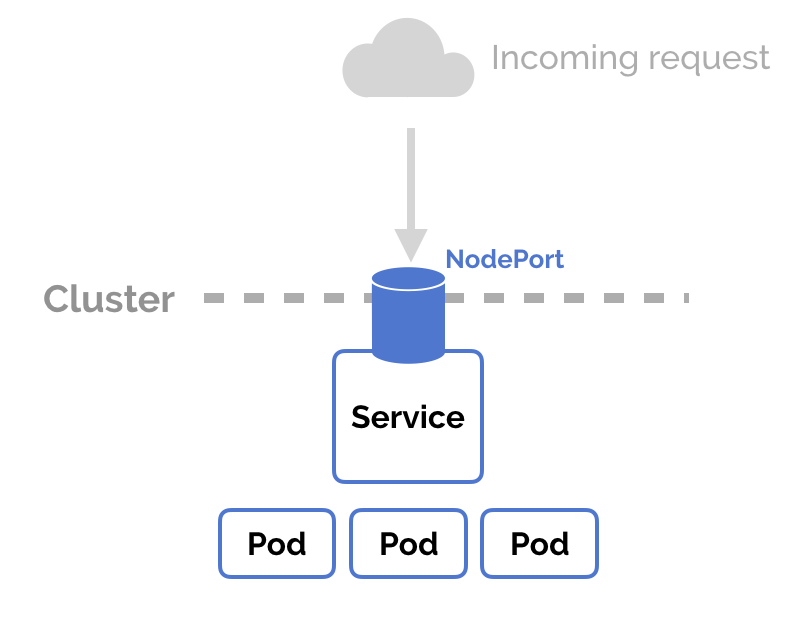
\includegraphics[totalheight=0.4\textheight]{service}
\end{center}
\subsubsection{Ingress network}
An ingress network exposes the services in the cluster to the outside network i.e. the clients. An ingress helps us in handling the outside traffic and directing them to the various services.\\
\begin{center}
	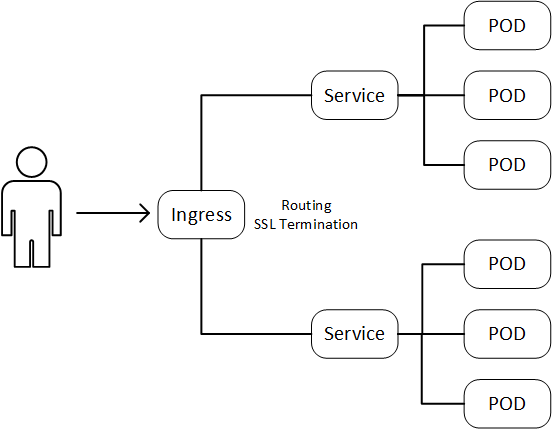
\includegraphics[totalheight=0.31\textheight]{ingress}
\end{center}
\subsection{Networking in Kubernetes}
Kubernetes supports a large number of network  plugins using different protocols. The type of networking to be used completely depends on the type of cluster you want to set up and your cluster requirements.\\\\
In a kubernetes network each pod is assigned its own IP address. Pods can communicate with pods, nodes and services in a node without NAT. \\\\
The networking in kubernetes can be broken down into majorly 4 parts :
\begin{enumerate}
	\item Container to container communication
	\item Pod to pod communication
	\item Pod to service communication
	\item Service to external Communication
\end{enumerate}
The major plugins used for achieving these communications are :
\subsubsection{Flannel}
Flannel is the simplest kubernetes network  which satisfies all kubernetes requirements. Flannel is basically an overlay network.
\begin{center}
	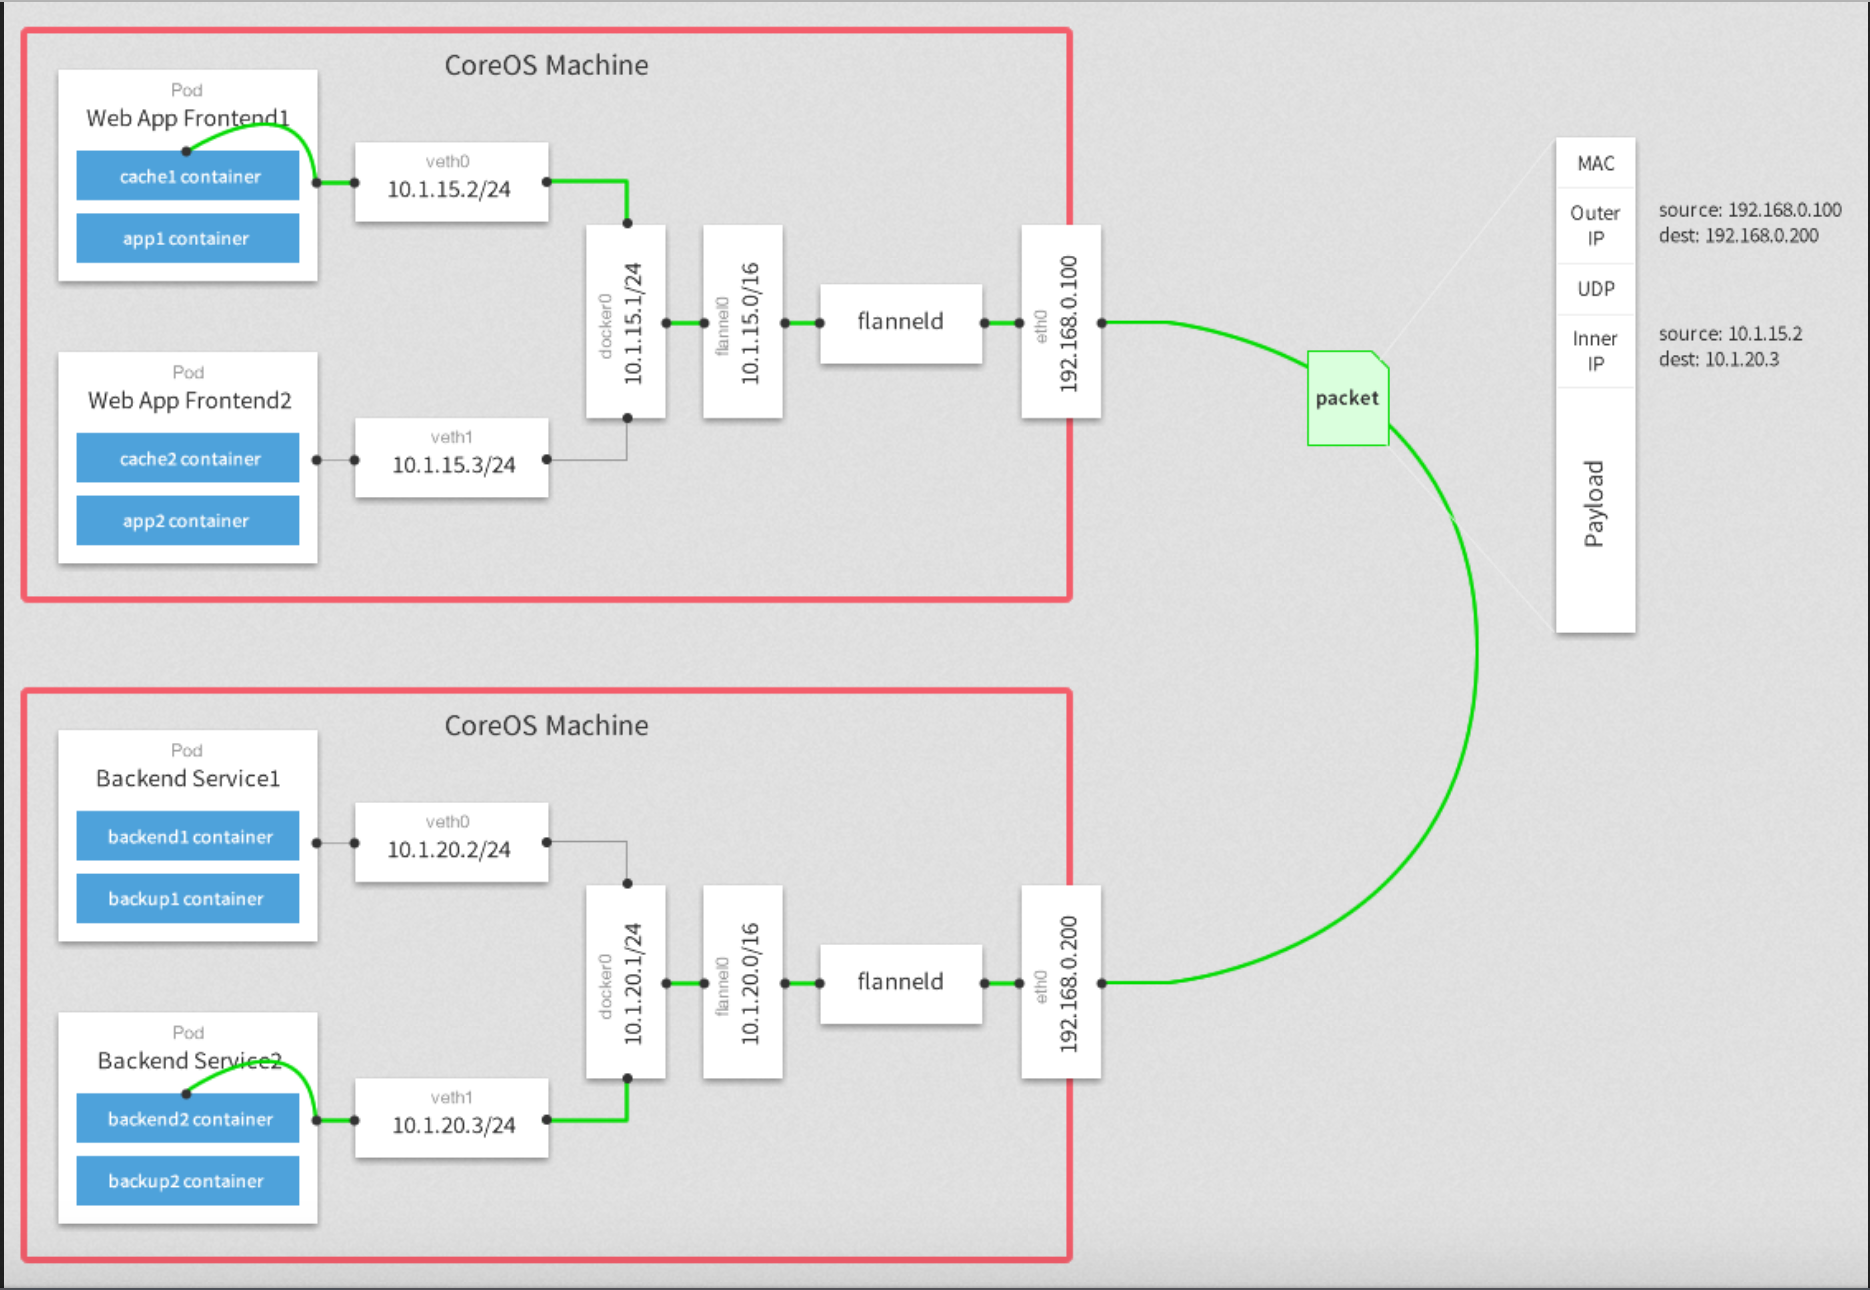
\includegraphics[totalheight=0.5\textheight, width=\textwidth]{flannel}
\end{center}
\subsubsection{Calico}
Calico provides a highly scalable networking and network policy solution for connecting Kubernetes pods based on the same IP networking principles as the internet, for both Linux and Windows. Calico can be deployed without encapsulation or overlays to provide high-performance, high-scale data center networking.
\begin{center}
	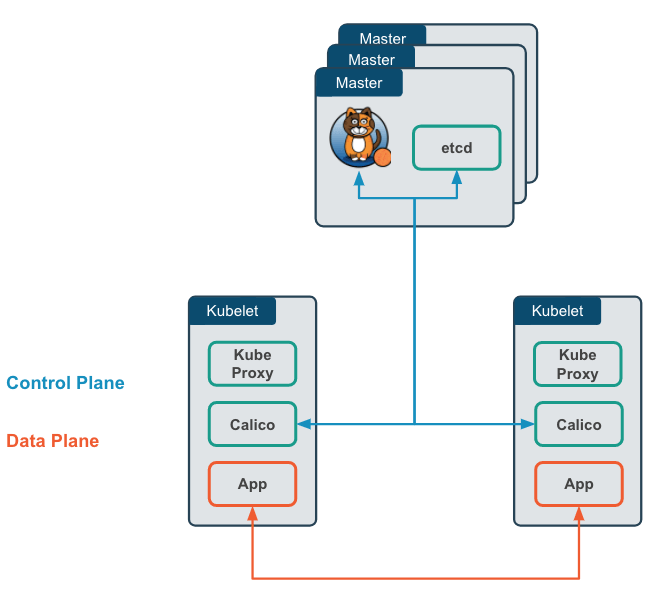
\includegraphics[totalheight=0.4\textheight]{calico}
\end{center}
\subsubsection{Weavenet}
Weavenet is a simple network for kubernetes and its hosted applications. Weave Net runs as a CNI plug in or stand-alone.
\begin{center}
	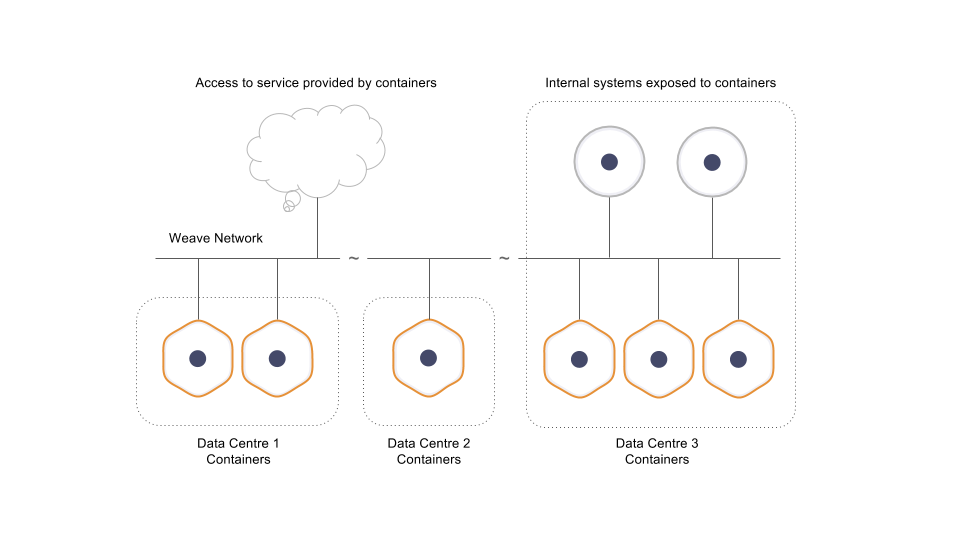
\includegraphics[totalheight=0.35\textheight]{weavenet}
\end{center}
In addition to these we have a lot of network plugins supported by kubernetes. A list of them can be found in the official documentation page of kubernetes (\href{https://kubernetes.io/docs/concepts/cluster-administration/networking/}{Networking in Kubernetes}).
\subsection{Prerequisites for running kubernetes}
\subsubsection{Disable Swap Space}
In order to set up a kubernetes cluster all nodes including master must have swap space disabled.
\begin{itemize}
	\item To disable swap space for current session run: \\
		  \textbf{\$ sudo swapoff -a}
	\item To permanently disable swap space go to /etc/fstab and comment the swap space line.
\end{itemize}
\subsubsection{Make IP static}
All nodes in cluster including master must have a static IP address.\\
In order to manually make the IP static add the following lines to the file /etc/network/interfaces:\\\\
auto wlo1\\
iface wlo1 inet static\\
address  YOUR\_IP\_ADDRESS
\subsection{Kubernetes setup}
\begin{enumerate}
	\item Install docker (follow the steps given \hyperref[sec:dockerinstall]{here} to successfully install docker).
	\item Enable docker to autostart during restart:\\
	\textbf{\$ sudo systemctl enable docker}
	\item Install curl:\\
	\textbf{\$ curl -s https://packages.cloud.google.com/apt/doc/apt-key.gpg $\vert$ sudo apt-key add}
	\item Add Google’s kubernetes repository:\\
	\textbf{\$ sudo apt-add-repository "deb http://apt.kubernetes.io/ kubernetes-xenial main"}
	\item Install kubeadm, kubectl and kubelet:\\
	\textbf{\$ sudo apt-get install kubeadm}\\
	\textbf{\$ sudo apt-get install kubectl}\\
	\textbf{\$ sudo apt-get install kubelet}
\end{enumerate}
\subsection{Setting up your Kubernetes cluster}
In order to set up your cluster first initialise your master with kubeadm:\\\\
\textbf{\$ kubeadm init  -{}-apiserver-advertise-address=YOUR\_IP\_ADDRESS    -{}-pod-network-cidr=40.196.0.0/16}\\\\
On successful execution of the command we get a join command for the worker nodes to join the cluster. Preserve this command to bring nodes into the cluster once the dashboard is created.\\\\
 You can also generate the join token by running the command :\\\\
 \textbf{\$ kubeadm token create}\\\\
 And the SHA256 key can be generated by running the command:\\\\
 \textbf{\$ openssl x509 -pubkey -in /etc/kubernetes/pki/ca.crt $|$ openssl rsa -pubin -outform der 2$>$/dev/null $|$ openssl dgst -sha256 -hex | sed 's/\string^.* //'}\\\\
 Now to bring any node into the cluster run the following command into the cluster after changing the IP with your master system’s IP address, token and SHA256 key with that generated by running the above command:\\\\
 \textbf{\$ kubeadm join IP\_OF\_MASTER:6443 -{}-token GENERATED\_TOKEN -{}-discovery-token-ca-cert-hash sha256:GENERATED\_HASH}\\\\
 Now once you have successfully initialised the cluster run the following commands :\\\\
 \textbf{
 \$ mkdir -p \$HOME/.kube\\
 \$ sudo cp -i /etc/kubernetes/admin.conf \$HOME/.kube/config\\
 \$ sudo chown \$(id -u):\$(id -g) \$HOME/.kube/config
}
\subsubsection{Setting up a pod network}
	i) To install and set up a calico pod network run the command :\\\\
	\textbf{\$ kubectl apply -f https://docs.projectcalico.org/v3.1/getting-started/kubernetes/\\installation/hosted/kubeadm/1.7/calico.yaml}\\\\
	ii) To install and set up flannel pod network run the command :\\\\
	\textbf{\$ sudo kubectl apply -f https://raw.githubusercontent.com/coreos/flannel/master/\\Documentation/kube-flannel.yml}\\\\
	There are a lot of plugins available that can be used as per the requirements. In this project we have used a calico pod network as CNI.\\
	Once the network is set up we need to install and host the dashboard on localhost.
\subsubsection{Setting up and hosting the dashboard}
	i) For installation and hosting in localhost : \\\\
	\textbf{\$ kubectl create -f https://raw.githubusercontent.com/kubernetes/dashboard/\\v1.8.3/src/deploy/recommended/kubernetes-dashboard.yaml}\\\\
	ii) For Creating service account:\\\\
	\textbf{\$ kubectl create serviceaccount dashboard -n default}\\\\
	iii) To add cluster binding rules to the dashboard:\\\\
	\textbf{\$ kubectl create clusterrolebinding dashboard-admin -n default 
		\\-{}-clusterrole=cluster-admin 
		\\-{}-serviceaccount=default:dashboard}\\\\
	iv) To generate token for login\\\\
	\textbf{\$ kubectl get secret \$(kubectl get serviceaccount dashboard\\ -o jsonpath="{.secrets[0].name}") -o jsonpath="{.data.token}" $|$ base64 -{}-decode}\\\\
	After the token is generated you can run the dashboard on localhost on port 8001(default). To bring up the dashboard run the command :\\\\
	\textbf{\$ kubectl proxy}\\\\
	Now you can visit the dashboard on the localhost:8001 at url:\\\\
	\href{http://localhost:8001/api/v1/namespaces/kube-system/services/https:kubernetes-dashboard:/proxy/}{http://localhost:8001/api/v1/namespaces/kube-system/services/https:kubernetes-\\dashboard:/proxy/}\\\\
	The dashboard can be accessed by entering the token generated. We can see the pods running, deployments, services and volumes created. We can also scale up and scale down the number of replicas.
	\subsubsection{Kubernetes commands for getting resource info}
	In order to get the complete details of  the pods via command line run the command :\\\\
	\textbf{\$ kubectl get pods -o wide -{}-all-namespaces}\\\\
	For viewing pods in default namespace run the command:\\\\
	\textbf{\$ kubectl get pods}\\\\
	Similarly for viewing deployments and services run the corresponding commands:\\\\
	\textbf{\$ kubectl get deployments}\\
	\textbf{\$ kubectl get services}\\\\
	So now the cluster is set up and we can create deployments for the running in the cluster. We can expose these deployments to endpoints via services and to external traffic by creating an ingress network.
	\subsection{Kubernetes API Server}
	Gateway to the Kubernetes cluster is Api server. It is a centralized system that is accessed by all users, automation, and components in the Kubernetes cluster. The API server implements a RESTful API over HTTP, performs all API operations, and is responsible for storing API objects into a persistent storage backend. This chapter covers the details of this operation.
	\begin{center}
		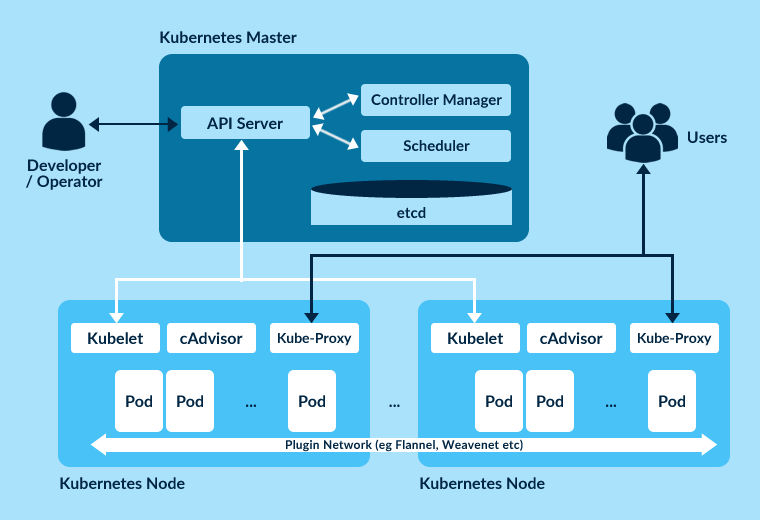
\includegraphics[totalheight=0.45\textheight]{kubernetesapiserver}
	\end{center}
	\subsubsection{Pieces of API Server}
	Kubernetes API server has three core functions:
	\begin{itemize}
		\item \textbf{API management:}\\\\
		In API management process, APIs are exposed and managed by the server.
		\item \textbf{Request processing:}\\\\
		Request processing processes individual API requests from a client.
		\item \textbf{Internal control loops:}\\\\
		Internal control loops has internals responsibilities for background operations necessary to the successful operation of the API server.
	\end{itemize}
\subsubsection{API Management}
The API server is an HTTP server—thus, every API request is an HTTP request. But the characteristics of those HTTP requests must be described so that the client and server know how to communicate. For the purposes of exploration, it’s great to have an API server actually up and running so that you can poke at it. You can either use an existing Kubernetes cluster that you have access to, or you can use the minikube tool for a local Kubernetes cluster. To make it easy to use the curl tool to explore the API server, run the kubectl tool in proxy mode to expose an unauthenticated API server on localhost:8001 using the following command:\\\\
\textbf{\$ kubectl proxy}
\subsection{Request Management}
The main aim of Api server is to receive and process API calls in form of HTTP request.\\
Type of request performed by Api server are following:
\begin{itemize}
	\item Get
	\item List
	\item Post
	\item Delete
\end{itemize}
\begin{center}
	\includegraphics*[totalheight=0.1\textheight]{kubereqman}
\end{center}
\subsection{ETCD}
A key-value storage for kubernetes backing store for all cluster data.
\subsection{Kube-Scheduler}
If there is a newly created pod which is not allocated any node then Kube-Scheduler select a node for them to run.
\subsection{Kube-Control-Manager}
Kube-Control-Manager is a component on master that runs controllers.
Each controller is a separate process but they are all merged.\\\\
These controllers include:
\begin{itemize}
	\item \textbf{Node controller:} Responsible for noticing and responding when nodes go down.
	\item \textbf{Replication controller:} Responsible for maintaining the correct number of pods for every replication controller object in the system.
	\item \textbf{Endpoints controller:} Populates the Endpoints object (that is, joins Services \& Pods).
	\item \textbf{Service Account \& Token Controllers:} Create default accounts and API access tokens for new namespaces.
\end{itemize}
\subsection{Converting docker-compose file to its Kubernetes equivalent}
Write text here
\subsubsection{Kompose}
Write text here
\subsubsection{Compose on Kubernetes}
Example of bulleted list
\begin{itemize}
 \item write point 1 here \cite{SRS1998}\cite{SimpleCCP-Windows}
 \item write point 2 here
 \item write point 3 here
\end{itemize}

Example of Numbered list
\begin{enumerate}
 \item Write point 1 here
 \item Write point 2 here
 \item write point 3 here
\end{enumerate}

\section{Tutor: An alternative}
Write text here

\section{Deployment}
\pagebreak

\section{Another Section name}
Write text here. Example of table.
\begin{table}[H]
\begin{center}
\begin{tabular}{|c|c|p{4cm}|}
 \hline
 \textbf{No.} & \textbf{Company} & \textbf{Operating System} \\
 \hline
 1 & Nokia & Symbian (S60, S40) \\
 \hline
 2 & Microsoft & Windows \\
 \hline
 3 & Apple Inc. & IOS \\
 \hline
 4 & Blackberry & Blackberry \\
 \hline
\end{tabular}
 \caption{Mobile Operating Systems}
 \end{center}
\end{table}

\subsection{Subsection}
Write text here


\section{Fifth Section name}
Write text here

\subsection{Subsection}
Write text here

\subsubsection{Sub-Sub-section}
Write text here

\bibliographystyle{ieeetr}
\bibliography{biblio}


\end{document}